\section{Literature Review}
There are several ways of designing and implementing Domain Specific Languages, each way having several merits and demerits. One of the most fundamental ways of classifying DSLs is Internal and External. \textbf{Internal DSLs} use the infrastructure of existing programming languages and build domain - specific constructs on top it. \textbf{External DSLs} are developed ground up and have separate infrastructure for lexical analysis, parsing, interpretation and compilation. The project was restricted to \textit{internal, embedded} DSLs in Scala.
\bigskip

\noindent
The areas covered under literature review include choice of programming language, choice of DSL design approach, different ways of performing tests and techniques to optimize DSLs in the compilation pipeline.
\bigskip

\subsection{Research Methodology}

The research methodology followed during the project involved reading relevant papers, reading industry best practices and white - papers and iteratively building a suitable solution. Each iteration was approximately two weeks long and involved getting feedback from the users.

\begin{figure}[H]
  \centering
    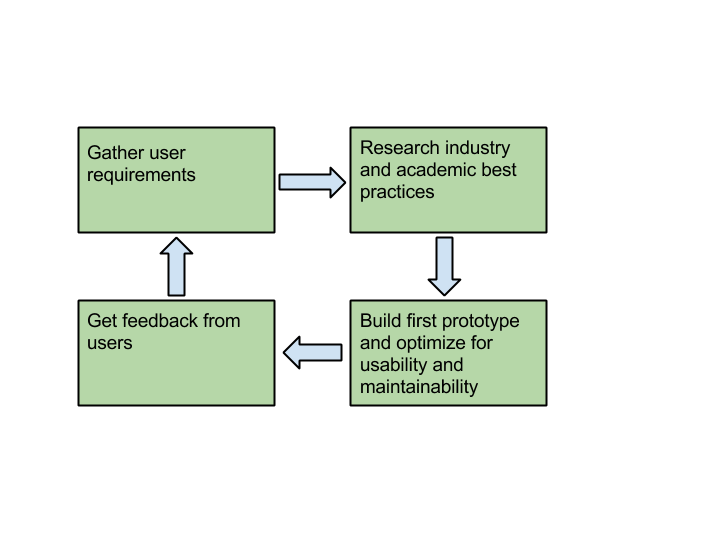
\includegraphics[height=300px]{figures/research.png}
  \caption{Research Methodology}
\end{figure}

\subsection{Testing Paradigms}
Release cycles and deployment cycles are becoming more and more frequent in the software engineering world and development teams are looking for reliable ways of testing their code's safety and functionality reliably and conveniently. Instituting an automated unit testing practice across a large software development team can be technically challenging and time consuming. Microsoft conducted a research study where a team of developers were instructed to write \textbf{unit tests} for all the functionality they wrote every 2 - 3 days. The bugs per unit of code were much fewer but there was a need for system level tests and integration tests \cite{unitTestingAtMicrosoft}. The chart below depicts the developer perception of the effectiveness of unit tests. The majority of Microsoft developers  are neutral towards unit testing.
\bigskip

\begin{figure}[H]
  \centering
    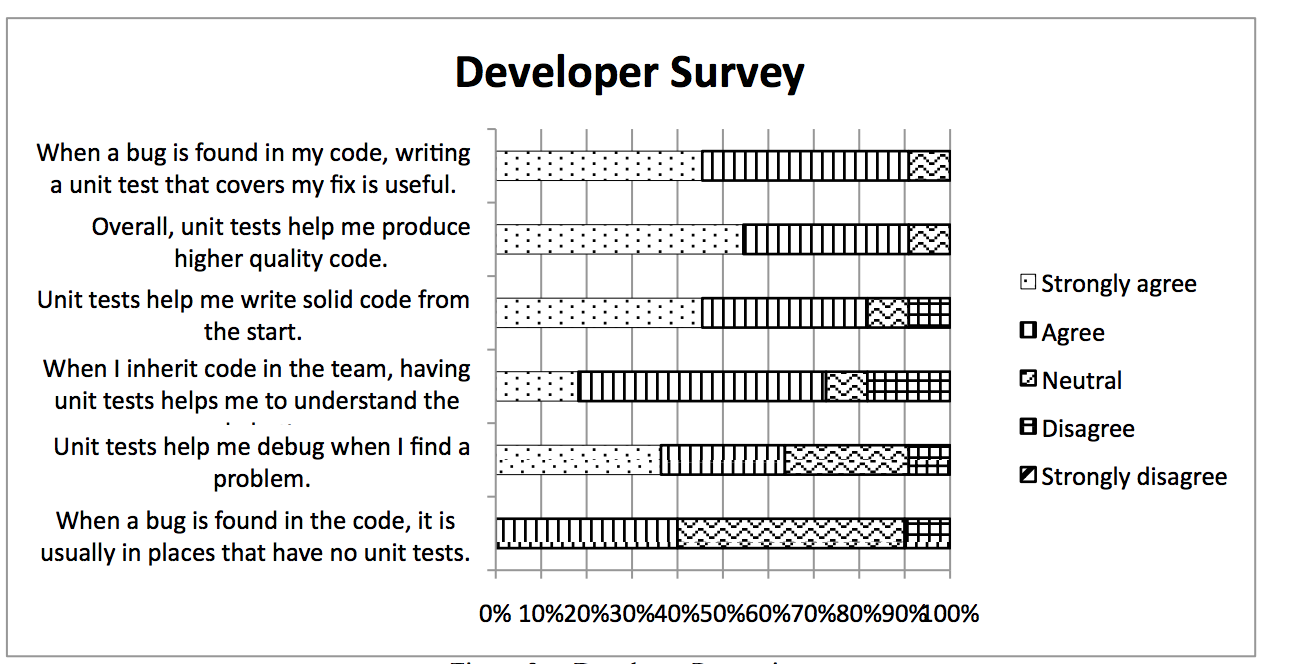
\includegraphics[height=200px]{figures/developer_perception.png}
  \caption{Developer Perception of the Effectiveness of Unit Testing}
\end{figure}

\noindent
In order to go beyond unit tests and perform functional tests at a system level, the DSL developed allows functional tests to be written for all kinds of domains. Since sometimes only the functionality of the software module is of primary concern, functional testing is used. Functional Testing is a testing method that emphasizes executing the functions and examination of their input and output data \cite{Hetzel88}. Given the high proliferation of frameworks like \textbf{JUnit, ScalaTest and NUnit} for unit testing, a DSL for functional testing on the system testing was developed during this project. Hetzel also emphasizes the importance of regression testing since software is built as a composition of third - party libraries and in - house components. This dictates that any minor change should lead to re - running tests on a unit level \cite{Hetzel88}. Therefore, the DSL developed has extensive support for \textbf{regression testing and reporting}.

\subsection{Domain Specific Language Design}
Ghosh discusses two approaches to constructing internal DSLs - \textbf{Embedded} and \textbf{Generative} \cite{dslsInAction}. Statically typed languages offer types as one of the means to abstract domain semantics and make the surface syntax of the DSL concise. Typed models come with a guarantee of some level of implicit consistency in the programming model. The biggest advantage of this technique is that because the DSL’s type system is embedded in the type system of the host language, the type system is automatically type-checked by the language compiler. This approach means that DSL users are able to use the IDE for debugging and tooling. In our System Testing DSL, this embedded DSL approach has been explored. 
\bigskip

\begin{figure}[H]
  \centering
    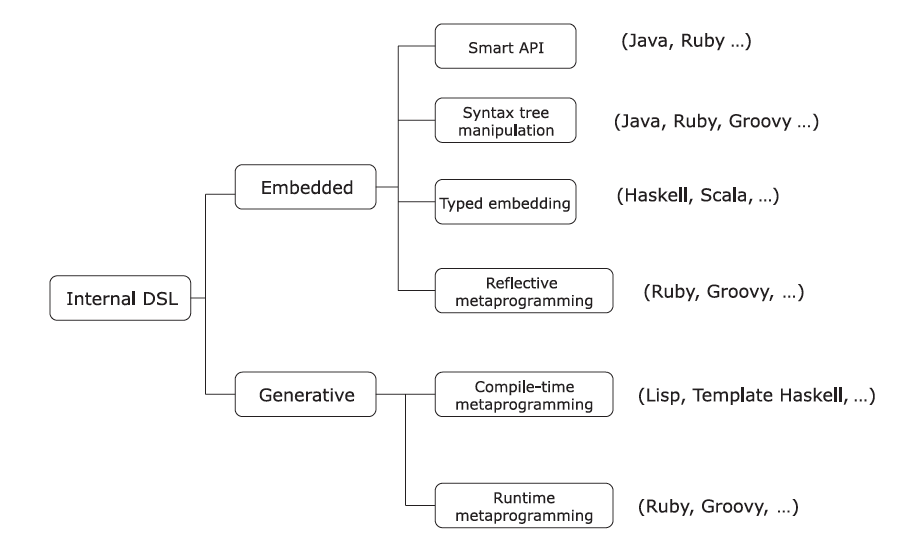
\includegraphics[height=250px]{figures/classification.png}
  \caption{Micro - classification of DSLs}
\end{figure}

\noindent
Languages like Haskell and Scala offer advanced static typing with type inference allowing DSL developers to write embedded DSLs without having to resort to code generation techniques, pre - processors or macros. As a DSL user, type abstractions can be composed directly. This is the approach that has been chosen while writing the System Testing DSL. Ghosh talks about using method chaining and fluent interfaces in DSL development as this gives a finished, declarative, natural language like feel \cite{fluentInterface}. The builder pattern is one more way in which DSL's can be made more expressive to the domain user. The builder pattern along with method chaining have been incorporated into the System Testing DSL to provide ease of use and expressiveness. More details on how this has been extensively applied is present in the \textit{design choices} section. 

\subsection{Lightweight Modular Staging: A run - time code generation approach}
Rompf and Odersky (2010) talk about an alternative approach to writing DSLs in Scala using a run - time code generation approach called lightweight modular staging \cite{lms}. This approach involves both a generative and an embedded approach. The DSL is provided as a library and involves run - time code generation in different stages. The approach is called \textbf{Light - Weight Modular Staging (LMS)}. The approach is lightweight because the whole framework is implemented as a library and the staged code is very shallowly embedded into the program generator. Some of the features of lightweight modular staging are described below:
\begin{itemize}
\item Immediate/deferred compilation of certain objects are distinguished by type
\item The Scala language is expressive enough to allow the framework to be implemented as a library
\item Staged code is “very shallowly” embedded into the program generator
\end{itemize}
\bigskip

\noindent
Lightweight modular staging provides many of the benefits of using a dedicated multi-stage programming language such as MetaOCaml, in particular concerning well-formedness and type safety, but goes beyond that in systematically preventing code duplication and providing a clean interface for incorporating generic and customized optimizations. However, after careful evaluation, this method was not chosen as the LMS project is still not mature enough, does not provide any advantages to the system testing domain and does not have tooling support.

\subsection{Delite: A framework for high - performance DSL's}
A third approach to writing embedded, high - performance DSLs conducted by Odersky built upon the concept of using lightweight modular staging. The research resulted in a framework called Delite \cite{delite}. Delite's compilation pipeline takes care of optimizing for target hardware such as multi - core processors, GPUs and computing clusters.

\begin{figure}[H]
  \centering
    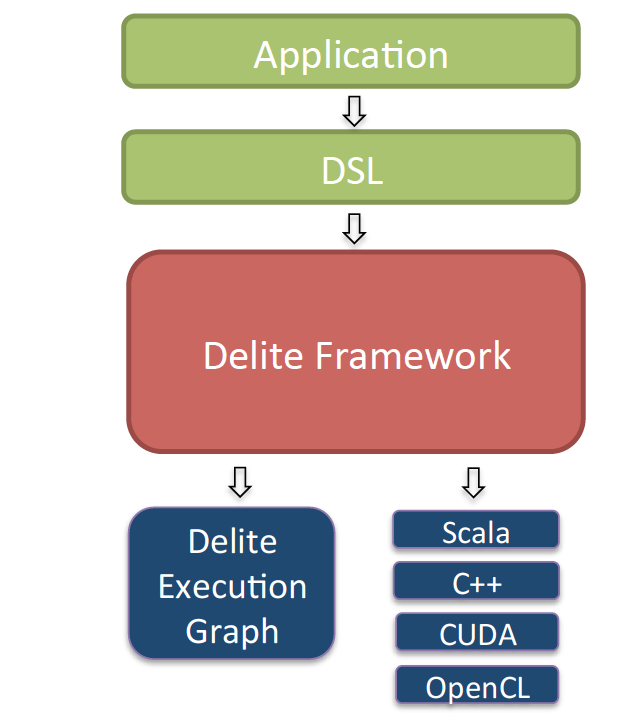
\includegraphics[width=170px]{figures/delite.png}
  \caption{Delite Framework Overview}
\end{figure}

\noindent
In the early stages of this project, the Delite framework was experimented with to gauge the suitability of the framework in everyday DSL development. However, due to the lack of sufficient tooling and documentation - the plans of using Delite were set aside.
\bigskip

\subsection{Scala programming language}
The \textbf{Scala} programming language was chosen as the host language for the DSL being developed. Scala is extremely well - suited for building embedded DSLs with custom syntax and rich type systems. Compiler features such as an \textbf{extensible type system, flexible syntax, type inference and static typing} are just some of the primary reasons for using Scala. According to the Scala specification, \textit{Scala is a statically typed multi-paradigm language that attempts to unify object-oriented and functional programming} \cite{scala}
\bigskip

\noindent
A recent paper published by Google comparing the performance of Scala, Java and Go show that although Scala has greater compilation times than Java and Go, the lines of code in Scala to achieve similar tasks are much lower than Java or Go. This is one more reason why Scala is suitable for DSL programming \cite{performanceComparison}.

\begin{figure}[H]
  \centering
    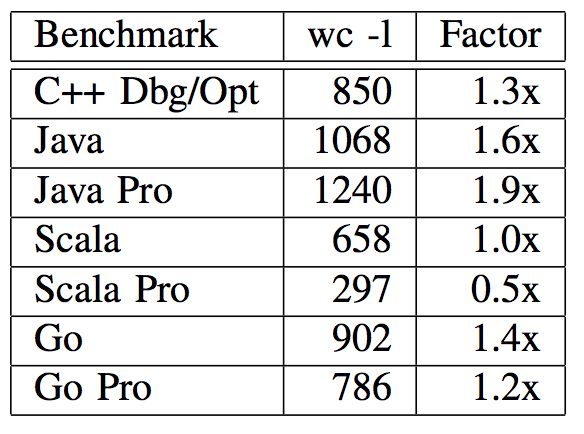
\includegraphics[height=150px]{figures/scala_loc.png}
  \caption{Comparison of Scala lines of code with other languages}
\end{figure}

\subsection{Python programming language}
Along with the two DSLs for system testing in Scala, a DSL was built for repository testing. This DSL was built in Python and is configured using YAML markup. Rewriting the DSL in Python provided a good opportunity to compare the differences in DSL development between a statically typed language like Scala and a dynamic language like Python.
\bigskip

\noindent
Python is a highly used high - level programming language with dynamic typing. It supports multiple programming paradigms such as object - oriented, imperative, functional and procedural. Python emphasizes the need for code to be human readable and expressive. The lines of code required to achieve something in Python is typically less than the number of lines required in Java or C \cite{pep}.
\bigskip

\noindent
The reference implementation of Python is CPython. CPython is written in and is a byte - code interpreter. CPython is the most widely used implementation and is marked as production quality. However, CPython does have certain issues with concurrency leading to certain drawbacks of the implementation. This can be attributed to the \textbf{Global Interpreter Lock (GIL)} \cite{cpython}. The GIL disables multiple Python threads within one Python process thereby restricting concurrency support.
\bigskip

\noindent
The DSLs developed during this project did not require emphasis on concurrency and therefore, Python could be used for comparison purposes. The reasons for choosing python for comparison with Scala were:
\begin{itemize}
\item It is a dynamic language and well - suited for such systems
\item It is close to the operating system and can easily make system calls
\item It supports \textbf{object orientation} leading to a more modular design \cite{python}
\end{itemize}

\begin{figure}[H]
  \centering
    
\includegraphics[height=150px]{figures/python_lang.png}
  \caption{Python}
\end{figure}
After consideration of these factors, \textbf{Python} was chosen to build the system with a configuration file written in YAML.

\subsection{Approach Chosen}
Out of the three DSL design approaches explored - \textbf{DSL development using embedded types}, \textbf{Lightweight Modular Staging} and \textbf{The Delite Framework}, the first one was chosen for developing the System Testing DSL. This \textbf{Embedded DSL} approach was chosen for the following reasons:
\begin{itemize}
\item This approach would lead to greater type - safety due to compile time type checking
\item Reduces the time overhead of run - time code generation
\item Emphasis could be placed on modelling the domain and producing meaningful semantics
\item Ease of integration with application code as the DSLs are implemented as libraries.
\end{itemize}
\bigskip

\noindent
\textbf{Scala} was chosen as the language for writing both DSLs. A dynamic version of the second DSL was also written in Python to compare with the primary DSL in Scala. Various other nuances such as \textbf{choice of configuration media} and \textbf{build and deployment choices} were also explored while writing the DSLs. These design choices and the reasons for making them are described in the \textbf{Design Choices} section.

\newpage

